\documentclass{beamer}
\mode<presentation>
 \usetheme{CambridgeUS}
%\usepackage{bussproofs}
%\usetheme{Singapore}
%\usecolortheme{lily}
  %%\usetheme{Logictheme} %nothing else
  %\setbeamertemplate{footline}[frame number]
  
%%\usepackage{bussproofs}
%%\usepackage[latin1]{inputenc} 
%%\newcommand{\mypause}{}
%%\newcommand{\mypause}{\pause}


%\institute[Madrid]{Swansea Railway Verification Group, Critical Software Technologies, Invensys Rail\\ \quad}
%\title[Logic in Railway Verification]{Application of Logic to the Verification\\ of Railway Control Systems}
%\title[Surrey Workshop]{Modelling and Analyzing the European Rail Traffic Management %System (ERTMS)}
\title[Modelling of Railway Control Systems]{Modelling of Railway Control Systems  -  \\ Safety and Performance}

\author[Monika Seisenberger]{Monika Seisenberger}
\date[Pretoria, 22 April 2015]{Swansea Railway Verification Group\\[1em]  Pretoria, 22 April 2015}
\institute[Swansea University]{Joint work with Andrew Lawrence, Ulrich Berger,  Phil James, Markus Roggenbach}

\usepackage{tikz}
\usepackage{graphicx}
\newcommand{\Red}{\mathbf{Red}}
\input{../14genua/sdmacros.tex}
\input{../14genua/macrosAL.tex}

\newtheorem{mydef}{Definition}
\newtheorem{myremark}{Remark}
\newcommand{\ednote}[1]{{\bf #1}}
\newcommand{\fig}[1]{Fig.~\ref{fig:#1}}
\newcommand{\Val}{{\rm Val}}
\newcommand{\unprime}{{\rm unprime}}
\newcommand{\Vars}{{\rm Vars}}


\newcommand{\rungStart}{
  %% Draw a -
  -- ++(2,0)
}

\newcommand{\contact}[1]{
  %% Draw a -
  -- ++(1,0)
  %% Draw ]
  +(-0.1, 0.5) -- +(0, 0.5) -- +(0, -0.5)  -- +(-0.1, -0.5)
  %% Move across
  ++(0.4, 0)
  %% Draw text above
  +(0,0.8) node{#1}
  %% Move across
  ++(0.4, 0)
  %% Draw [
  +(0.1, 0.5) -- +(0, 0.5) -- +(0, -0.5)  -- +(0.1, -0.5)
  %% Reset to current point
  ++(0, 0) --
  %% Draw a -
  ++(1,0) 
}


\newcommand{\closedContact}[1]{
  %% Draw a -
  -- ++(1,0)
  %% Draw ]
  +(-0.1, 0.5) -- +(0, 0.5) -- +(0, -0.5)  -- +(-0.1, -0.5)
  %% Move across
  ++(0.4, 0)
  %% Draw text above
  +(0,0.8) node{#1}
  %% Draw close i.e. /
  +(-0.2, -0.5) -- +(0.2, 0.5)
  %% Reset to current point (i.e. middle)
  ++(0, 0)
  %% Move across
  ++(0.4, 0)
  %% Draw [
  +(0.1, 0.5) -- +(0, 0.5) -- +(0, -0.5)  -- +(0.1, -0.5)
  %% Reset to current point
  ++(0, 0) --
  %% Draw a -
  ++(1,0) 
}

\newcommand{\coil}[1]{
   %% Draw a -
  -- ++(1,0)
  %% Move to end of -
  +(0.5,-0.5)
  %% Draw arc (
  arc (270:90:0.5cm)
  %% Move across
  ++(0.3, 0)
  %% Draw text above
  +(0,0.3) node{#1}
  %% Reset
  +(0.3,-1)
  %% Draw Arc )
  arc (-90:90:0.5cm)
  %% Move to center of )
  ++(0.5,-0.5)
  %% Finish Path
  ;
}


\newcommand{\nodeLink}[1]{
  %% Draw a -
  -- ++(0.5,0) node[inner sep=0pt, minimum size=0pt] (#1){};
}

\newcommand{\nodeLinkInline}[1]{
  %% Draw a -
  -- ++(0.5,0) node[inner sep=0pt, minimum size=0pt] (#1){} -- ++(0.5,0) 
}


\newcommand\boxAngle{150}

\newcommand{\mybox}[5]{ 
  %% #1 = Width, #2 = Height, #3 = Depth, #4 = x, #5 = y
  %% Front face
  \draw  (#4,#5) rectangle +(#1,#2);
  %% Draw side
  \draw [fill=gray!25] (#4,#5) -- ++(\boxAngle:#3) -- ++(0,#2) -- ++(\boxAngle:-#3);
  %% Draw top
  \draw [fill=gray!50] (#4,#5) ++(0,#2) -- ++(\boxAngle:#3) -- ++(#1,0) -- ++(\boxAngle:-#3);
}

\tikzstyle{myArrow}=[draw,->, line width=1.5pt]





\begin{document}

\begin{frame}
  \titlepage
\end{frame}


\begin{frame}

\frametitle{Overview:  Modelling of Railway Control Systems }

\medskip

\begin{center}
To investigate how a Centralized Traffic Control System, \\
the European Rail Traffic Management System (ERTMS) \\
can be modelled and verified using the Real-Time-Maude system
\end{center}
%\pause

\medskip

Overview:

%\begin{itemize}
%  \item \underline{Part I:} ERTMS -- what it is
% \item \underline{Part II:} ERTMS -- how it works
%  \item \underline{Part III:} Generic Modelling: ERTMS as a hybrid automaton
%  \item \underline{Part IV:} Encoding in Real-Time Maude   
%  \item \underline{Part V:} Verification \& simulation results
%\end{itemize}

\begin{itemize}
  \item \underline{Part I:} ERTMS -- what it is 
  \item \underline{Part II:} ERTMS -- how it works
  \item \underline{Part II:} Generic Modelling: ERTMS as a hybrid automaton
  \item \underline{Part I:} Encoding in Real-Time Maude   
  \item \underline{Part V:} Verification \& simulation results
\end{itemize}

\bigskip

\end{frame}

\section{ERTMS -- what it is}

%\begin{frame}
%\begin{center}
%{\Large ERTMS -- what it is}
%\end{center}

%\end{frame}



\begin{frame}

\frametitle{European Rail Traffic Management System (ERTMS) I}

What it is:
\begin{itemize}

\item
%European standard of signalling, control and train protection 
Standard of signalling, control and train protection

\item
to replace the many incompatible safety systems (20!) currently used by
European railways

\item 
offers possibility for traffic management

\item Originally designed for Europe, has rapidly become a global standard.

\item Switzerland: 1200km.

\item China: 8000km

\item UK: Cambrian Coast Line, 215km, (single track line to Gregynog!)

\item SA: Gautrain Rapid Rail Link, 80km 

\item SA: Spoornet ORE Export Line -Sishen to Saldanha, 861km , freight train line.
\end{itemize}




\end{frame}



\begin{frame}

\frametitle{European Rail Traffic Management System (ERTMS) II}

What it shall achieve:
\begin{itemize}

\item 
interoperability

\item
ease of maintenance (less track equipment)

\item 
high capacity

\end{itemize}

\bigskip\bigskip

Open research questions include:
\begin{enumerate}

\item
How can safety be verified? 

\item
How can capacity be measured and improved?

\item
How can reliability be measured and estimated?

\end{enumerate}

Here: 1 and, partially, 2.

\end{frame}

\section{ERTMS -- how it works}

%\begin{frame}
%\begin{center}
%{\Large ERTMS -- how it works}
%\end{center}
%\end{frame}


\begin{frame}
\frametitle{System components of ERTMS, level 2}
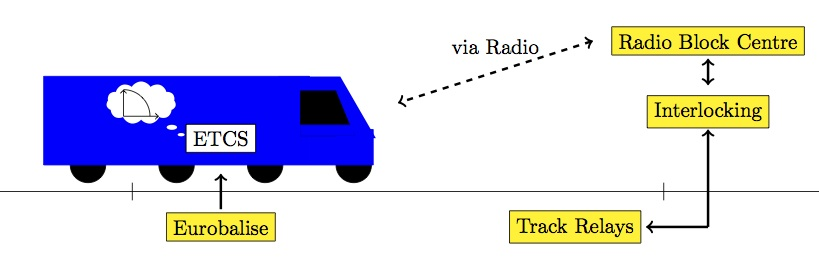
\includegraphics[scale =0.8]{ftscstalk/ETCSlevel2}
\end{frame}

\begin{frame}
\frametitle{Data in the ERTMS, level 2}
\begin{itemize}
\item Trains send position and speed (continuous data) and request \alert{Movement Autorities} from the RBC.

 
\item The radio block processor (RBC) consults with the interlocking and
grants or denies  a \alert{movement
  authority} (MA).

\medskip

\item The MA consists of a position on the track past which the train cannot
proceed called the end of authority (EoA) [and a static speed profile].

\medskip

\item Trains move on the track according to the physical laws of movement,
their breaking is controlled against a differential equation, their
acceleration follows a differential equation.

\medskip

\item Together the RBC, trains and the interlocking form a \alert{hybrid
  system}.
 \end{itemize}
\end{frame}


\begin{frame}
\frametitle{Information flow in ERTMS, level 2}
\begin{center}
%\includegraphics[scale=0.5]{ftscstalk/information-flow.png}
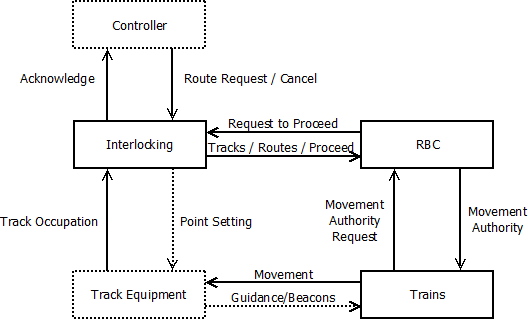
\includegraphics[scale=0.5]{wadtsiemens.png}
\end{center}
\end{frame}






\section{Generic modelling: ERTMS as a hybrid automaton}

\begin{frame}
\begin{center}
{\Large Generic modelling: ERTMS as a hybrid automaton}
\end{center}
\end{frame}




\begin{frame}
\frametitle{A model of a train with ERTMS equipment}
\begin{center}
\includegraphics[scale=0.55]{trainautomaton}
\end{center}
\end{frame}

\begin{frame}
\frametitle{ERTMS as a hybrid automaton: Interlocking and RBC}
\begin{center}
%\includegraphics[scale=0.21]{ftscstalk/trainautomata.jpg} %{\huge $ || $}
{\huge $ || $}
\includegraphics[scale=0.2]{ftscstalk/interlocking.png} {\huge $ || $}
\includegraphics[scale=0.2]{ftscstalk/rbc.png}
\end{center}
\end{frame}



\begin{frame}
\frametitle{Modelling the Interlocking}

\vspace*{-2cm}
%\begin{center}
\includegraphics[scale=0.7]{Interlocking}
%\end{center}
%%The interlocking checks whether the all tracksegments on the requested routes are free, and grants or denies.
\end{frame}



\begin{frame}
\frametitle{Modelling the RBC}
\vspace*{-3cm}
\begin{center}
\includegraphics[scale=0.6]{Rbc}
\end{center}
\end{frame}

\begin{frame}
\frametitle{Well-formedness of the hybrid automaton}

\bigskip

Modelling based on Henzinger, 2000.

\bigskip\bigskip

{\bf Theorem} This hybrid automaton is non-Zeno, \\ i.e. every finite
initialised trajectory in the labelled transition system defined by
the automaton has an infinite trajectory of which it is a prefix in
set of divergent initialized trajectories in the automaton.

\vfill

\end{frame}


\section{Encoding in Real-Time Maude}

%\begin{frame}
%\begin{center}{\Large Encoding in Real-Time Maude}
%\end{center}
%\end{frame}

\begin{frame}
\frametitle{Encoding in  Real-Time Maude}

Real-Time Maude (Peter C. \"Olveczky and Jos\'e Meseguer 2002) is a language and tool extending Maude, that allows for simulation and formal analysis of real-time and hybrid
systems.

\medskip

We make use of especially of its
\begin{itemize}

\item OO features

\item \alert{Discrete} time rewriting rules:
%
\begin{flushleft}
\texttt{  rl  [label] : \{Sys\} => \{Sys\} in time t .}\\
\texttt{  crl [label] : \{Sys\} => \{Sys\} in time t if C .} 
\end{flushleft}

%\item $\delta$ operator %describes system evolution in one time unit


\end{itemize}
\end{frame}
\begin{frame}[fragile]
\frametitle{Object Oriented Modelling}
\begin{verbatim}
mod CONFIGURATION is  
    *** basic object system sorts  
    sorts Object Msg Configuration .  
 
    *** construction of configurations  
    subsort Object Msg < Configuration .  
    op none : -> Configuration [ctor] .  
    op __ : Configuration Configuration -> Configuration  
         [ctor config assoc comm id: none] .
\end{verbatim}
\end{frame}

\begin{frame}[fragile]
\frametitle{Timed Progress of a train in state ``accelerating''}
\begin{verbatim}
crl [incspeed] : 
  {delta(< O : Train | state : acc, dist : DT, speed : S, 
                       ac : A, ma : MA, maxspeed : MAX >)
           REST}

   => 

  {pos(O,DT) 
   < O : Train |  dist : (DT + S), speed : S + A > 
   REST
  } 
  if S + A < MAX and ... .
\end{verbatim}
\end{frame}



\begin{frame}[fragile]
\frametitle{Message consumption for the RBC in state ``wait''}
\begin{verbatim}
rl [rbcgrant]:
  { grant(N) 
    <O : RBC | state : wait, lasttrain : T1, ma : MAP1 > 
    REST
  } 

=>

  { <O : RBC | state : rbcidle, 
               ma : insert(T1,endoftrack(N),MAP1) >
    grantma(T1, endoftrack(N)) 
    REST
  } .
\end{verbatim}
\end{frame}




\begin{frame}[fragile]
\frametitle{$\delta$ operator -- by {\"O}lveczky and Thorvaldsen, 2007}

\begin{verbatim}
op delta : Configuration -> Configuration . 
vars CON CON1 CON2 : Configuration . 
var OCREST : ObjectConfiguration .


rl [timetrans] : {OCREST} => {delta(OCREST)} in time 1 .
rl [delta] : delta(CON1 CON2) => delta(CON1) delta(CON2) .

--- mte = maximal time elapse
rl [mte] : {CON} => {delta(CON)} in time 1 if mte (CON) >= 1 .  

eq mte(none) = INF 
eq mte(CON1 CON2) = min(mte(CON1), mte(CON2)).
eg mte (MSG) = 0
eg mte (<    >) = ....
\end{verbatim}
\end{frame}










\section{Verification \& simulation results}

\begin{frame}
\begin{center}
{\Large Verification \& simulation results}
\end{center}
\end{frame}


\begin{frame}
\frametitle{First examples with 2 trains in each scenario}

\begin{center}
\begin{tabular}{cc}
\includegraphics[scale=0.25]{ftscstalk/pentagon.png} &
\includegraphics[scale=0.2]{ftscstalk/junction.png} \\
Pentagon-Example & Junction
\end{tabular}
\end{center}

\end{frame}



\begin{frame}
\frametitle{Train speed / distance over time -- Pentagon example}

\begin{center}
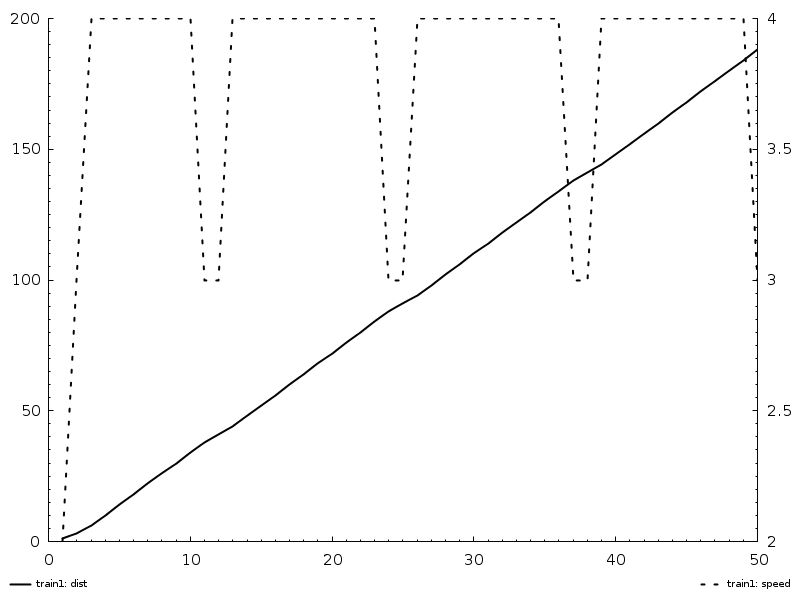
\includegraphics[scale=0.30]{ftscstalk/t1graph} 
\end{center}

\end{frame}

\begin{frame}
\frametitle{Train speed / distance over time -- Pentagon, 2nd train}

\begin{center}
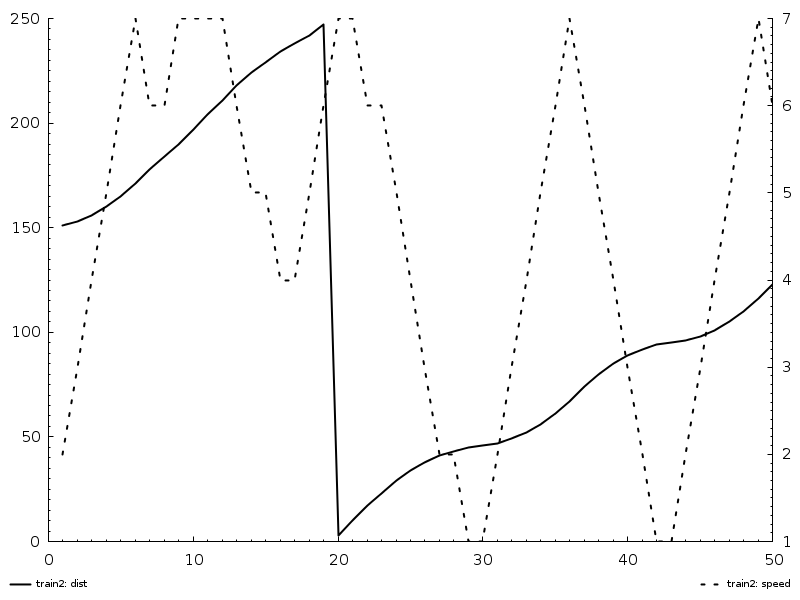
\includegraphics[scale=0.30]{ftscstalk/t2graph} 
\end{center}

\end{frame}

\begin{frame}
\frametitle{Comparison of both trains}
\begin{center}
\includegraphics[scale=0.30]{ftscstalk/t1t2graph241014} 
\end{center}

\end{frame}






\begin{frame}
\frametitle{Safety-Verification by applying Real-Time Maude
  Model-checking for Linear Temporal Logic}

Pentagon Example - 2 trains:
\begin{itemize}
\item
no overlapping MA in the first 100 time units
-- takes 91 secs
\end{itemize}

\bigskip
%Pentagon Example - 2 trains - tracklength 5000 - speed 120/70
%\begin{itemize}
%\item
%no overlapping MA in the first 70 time units
%-- takes 79 secs
%\end{itemize}

%\bigskip\bigskip

Junction - 2 trains:
\begin{itemize}
\item
no overlapping MA -- takes 7 secs

\item 
no derailment  -- takes 6 secs

\end{itemize}

\pause
\bigskip

We also compared with realistic tracklengths of 5000 - speed 120/70

\medskip

Pentagon Example - 2 trains:
\begin{itemize}
\item
no overlapping MA in the first 70 time units -- takes 79 secs
\end{itemize}
\end{frame}

\section{}


\begin{frame}
\frametitle{Ongoing work: Modelling and Verification}
\begin{itemize}
\item Modelling of  the controller: \\
Knows of trains routes, max speed of each train, initializes trains.\\
$\to $ Route setting, interaction with interlocking.\\


\bigskip
\item Generic track plans, control tables, release tables. 



\bigskip

\item Scenarios that lead to counter examples.

\bigskip
\item Limits of Model checking.

\bigskip

\item Review of assumptions: maximal progress assumption.

\bigskip

\item Completeness of modelling approach
\end{itemize}

\end{frame}


%\begin{frame}
%\frametitle{Modelling of a  simple Controller}
%Controller currently acts as scheduler for second example. Class with three parameters: 
%\begin{itemize}
%\item \texttt{trainorder}: stores a list of trains that are going to enter the track.

%\item \texttt{trainmax}: stores the maximum speed for each train.

%\item \texttt{trainroute}: stores the route of each train. 
%\end{itemize}

%\bigskip
%The controller sends request messages to the rbc that allows the train to enter.
%If granted, the train is removed from \texttt{trainorder}, and a train object is generated.
%A message is sent to the interlocking that the initial trainsegement is occupied.
%\end{frame}






\begin{frame}
\frametitle{Conclusion \& Future Work}


\begin{itemize}
%\item Demonstrated various techniques to verify  and simulate Railway control systems.



\item Our modelling approach works and is rich enough it to analyze ERTMS for
  important safety and capacity properties.

\item Real-Time Maude offers a competitive framework for modelling \&
 analysing ERTMS.
\medskip

%\item Extracted a SAT solver, sound and complete.
%\item Demonstrated that efficiency considerations can be taken into account at the proof level.

\end{itemize} %\pause


Future Work:
\begin{itemize}
%\item Formalize the relation between hybrid automaton and its discrete
%  approximation in Real-Time Maude.


\item Enrich the modelling to capture more aspects of ERTMS.
\item Develop the timed simulations towards capacity measures.


\bigskip

\item Aside: Final year student - Automatic translation of Ladderlogic into Real-Time Maude

%\item Further optimize the extracted SAT solver; takle a different class of problems.

\end{itemize}

\end{frame}

\end{document}
\begin{frame}
\frametitle{References}    
 
%Specification Implementation Verification Method:

  \begin{thebibliography}{10}    
  \beamertemplatearticlebibitems
  \bibitem{} James, P., Lawrence, A.,  Moller, F., Roggenbach, M., Seisenberger, M. and Setzer, A.Chadwick, S. ,P. Kanso, K., :
\newblock{\em  Verification of solid state interlocking programs.}
\newblock In SEFM'13, LNCS 8368, Springer 2014.
\end{thebibliography} 

\bigskip
%Extraction of SAT and Resolution algorithm:

\begin{thebibliography}{10}    
  \beamertemplatearticlebibitems
  \bibitem{}
    Berger, U.,  Lawrence, A., Nordvall Forsberg, F. , Seisenberger, M. 
    \newblock {\em Extraction of Verified Decision Procedures}. LMCS, to appear. 

\bigskip

\bibitem{} Lawrence, A, Berger, U. , James, P., Roggenbach, M., Seisenberger, M.
\newblock {\em Modelling and Analysing the European Rail Traffic Control System}
\newblock FTSCS, 2014.

\end{thebibliography}
\end{frame}



\end{document}

\begin{frame}

\frametitle{European Rail Traffic Management System (ERTMS) II}

Formal methods and ERTMS:
\begin{itemize}

\item
EuRailCheck (2009): \\ suggested methodology and tools for
formalization and validation of the standard.

\item
Open ETCS Project (ongoing): \\ works towards an integrated framework for
modelling, development, implementation and testing of the standard.

\end{itemize}

Open research questions include:
\begin{enumerate}

\item
How can safety be verified? 

\item
How can capacity be measured and improved?

\item
How can reliability be measured and estimated?

\end{enumerate}

Here: 1 and, partially, 2.

\end{frame}

\section{Modelling and Analyzing ERTMS}

%\begin{frame}
%\begin{center}
%{\Large ERTMS -- how it works}
%\end{center}
%\end{frame}
